\documentclass[a4paper,11pt]{article}
% ---- graphiques
\usepackage[pdftex]{graphicx}

% for latex2html
\usepackage{html}

% for accents
\usepackage[latin1]{inputenc}

% ---- inclusion de codes
\usepackage{listings}
\lstset{showstringspaces=false,frame=trBL,frameround=tttt,tabsize=4,basicstyle=\tiny,breaklines=true,breakatwhitespace=true}
\lstdefinestyle{bash}{language=bash}
\lstdefinestyle{Perl}{language=Perl}
\lstdefinestyle{C++}{language=C++}
\lstdefinestyle{DTD}{language=XML}
\lstdefinestyle{XML}{language=XML,usekeywordsintag=false,markfirstintag=true}
%begin{latexonly}
\newcommand{\includecode}[2]{
\lstinputlisting[style=#1]{#2}
}
%end{latexonly}
\begin{htmlonly}
\newcommand{\includecode}[2]{  \htmladdnormallink{#2}{../../#2} }
\end{htmlonly}
%\lstnewenvironment{code}{}{}
\lstnewenvironment{code_bash}{\lstset{style=bash}}{}
\lstnewenvironment{code_perl}{\lstset{style=Perl}}{}
\lstnewenvironment{code_cpp}{\lstset{style=C++}}{}
\lstnewenvironment{code_dtd}{\lstset{style=DTD}}{}
\lstnewenvironment{code_xml}{\lstset{style=XML}}{}

\newcommand{\textcode}[1]{{\small {\tt #1}}}




\newcommand{\sofa}{SOFA }
\newcommand{\todo}[1]{}
\newcommand{\eg}{\textit{e.g.} }


% macros mathematiques
\newcommand{\ma}[1]{\ensuremath{\mathbf {#1}}}
\newcommand{\ve}[1]{\ensuremath{\mathbf {#1}}}

\usepackage{amsmath}
\usepackage{amsfonts}
\usepackage{amssymb}

% character styles
\newcommand{\bm}[1]{\ensuremath{\mathbf{{#1}}}}
\newcommand{\mcal}[1]{\mbox{$\mathcal #1$}} % rondes math
\newcommand{\bmcal}[1]{\mbox{\boldmath $\mathcal #1$}} % rondes grasses math
\newcommand{\ensemble}[1]{\mbox{$\mathbb{#1}$}}
\newcommand{\RRR}{\mbox{$\ensemble{R}^3$}} 


% d�finitions
\newcommand{\definition}[2]{\index{#1}{\bf #1}: #2}
\newcommand{\voc}[1]{\index{#1}#1}
\newcommand{\bvoc}[1]{\index{#1}{\bf #1}}

% misc
\newcommand{\EV}[1]{\stackrel{\rightarrow}{#1}}  % espace vectoriel
\newcommand{\EA}[1]{#1}                          % espace affine

% vectors, matrices
%\newcommand{\point}[1]{\mbox{$#1$}}          % un point
\newcommand{\point}[1]{\ensuremath{#1}}          % un point
\newcommand{\mat}[1]{\bm{#1}}         % matrice
\newcommand{\matnm}[3]{\bm{#1_{#2\times #3}}}  % matrice n lignes , m colonnes
\newcommand{\vect}[1]{\bm{#1}}        % vecteur 
%\newcommand{\vecf}[1]{\stackrel{\rightarrow}{#1}}  % vecteur avec fleche
\newcommand{\vecf}[1]{\mbox{$\overrightarrow{#1}$}}  % vecteur avec fleche
\newcommand{\ident}[1]{\bm{I_{#1}}}   % identit� en dimension n
\newcommand{\inv}[1]{#1^{-1}}         % matrice inverse
\newcommand{\psinv}[1]{#1^{+}}        % matrice pseudo-inverse
\newcommand{\transp}[1]{#1^T}         % transpos�e de 1
\newcommand{\trace}[1]{tr(#1)}        % trace
\newcommand{\deter}[1]{\mbox{$|#1|$}}       % determinant
\newcommand{\oppvec}[1]{\mbox{$\left( \vect {#1} \wedge \right)$}}  % operateur matriciel de produit vectoriel

% bases, reperes
\newcommand{\vecin}[2]{\mbox{${}^{#2}#1$}}    % vecteur 1 dans repere 2
\newcommand{\Base}[1]{\ensuremath{\mathcal B_{#1}}} % Symbole du repere 1
\newcommand{\chbase}[3]{\mbox{${}_{#2}^{#3}\mat{#1}$}}  % operateur 1 fait le passage de la base 3 vers la base 2
%\newcommand{\pchbase}[2]{\chbase{\mat{B}}{#1}{#2}}  % matrice de passage de la base 2 vers la base 1
\newcommand{\pchbase}[2]{\chbase{B}{#1}{#2}}  % matrice de passage de la base 2 vers la base 1
\newcommand{\Rep}[1]{\ensuremath{\mathcal R_{#1}}} % Symbole du repere 1
\newcommand{\rep}[1]{\Rep{#1}}                 % Symbole du repere 1
%\newcommand{\pchrep}[2]{\chbase{\mat{F}}{#1}{#2}}  % matrice de passage du repere 1 vers le repere 2, F comme Frame
\newcommand{\pchrep}[2]{\chbase{\bm{C}}{#1}{#2}}  % matrice de passage du repere 2 vers le repere 1

%% Operateur de passage du repere 1 par rapport a 2
%\newcommand{\ChgRep}[2]{\mbox{\boldmath $R_{#1}^{#2}$}}

% rotations	
%\newcommand{\rot}[2]{\mbox{$\mat{R}_{#1,#2}$}}      % rotation vectorielle
\newcommand{\rot}[2]{\ensuremath{\mat{R}_{#1,#2}}}      % rotation vectorielle
\newcommand{\rota}[3]{\mbox{$\mat{R}_{#1,#2,#3}$}}  % rotation affine

% translation
\newcommand{\trans}[2]{\mbox{$\chbase{\vect{t}}{#1}{#2}$}} % passage de #1 vers #2 par une translation, ou translation du repere #2 par rapport au repere #1

% vitesses et acc�l�rations
\newcommand{\VRep}[2]{\mbox{\boldmath $\dot R_{#1}^{#2}$}} % vitesse du repere 1 par rapport a 2 
%\newcommand{\Point}[2]{\mbox{\boldmath ${#1}^{#2}$}}  % Coordonnees d'un point 1 dans un repere 2
\newcommand{\Point}[2]{\mbox{$\vecin{\bm{#1}}{#2}$}}  % Coordonnees d'un point 1 dans un repere 2
\newcommand{\VPoint}[2]{\mbox{\boldmath ${\dot #1}_{/#2}$}} % Vitesse d'un point par rapport � un repere
\newcommand{\APoint}[2]{\mbox{\boldmath ${\ddot #1}_{/#2}$}} % Acceleration d'un point par rapport � un repere

% cinematique du solide
\newcommand{\derivedans}[2]{\mbox{$\dot{#1}^{(#2)}$}}  % derivee du vecteur 1 dans repere 2
\newcommand{\fixedans}[2]{\mbox{$#1_{\in #2}$}}        % vecteur 1 fixe dans repere 2
\newcommand{\vecom}{\mbox{$\bm{\Omega}$}}  % omega de 1 par rapport a 2
\newcommand{\vecrot}[2]{\mbox{$\vecom_{#1/#2}$}}  % omega de 1 par rapport a 2
\newcommand{\accrot}[2]{\mbox{$\dot{\vecom}_{#1/#2}$}}  % omega de 1 par rapport a 2
\newcommand{\vfdans}[3]{\mbox{$\vec V^{#2/#3}_{#1}$}}    % vitesse de 1 fixe dans 2 par rapport a 3
\newcommand{\afdans}[3]{\mbox{$\vec \Gamma^{#2/#3}_{#1}$}}    % acceleration de 1 fixe dans 2 par rapport a 3
\newcommand{\vmdans}[2]{\mbox{$\vec V^{/{#2}}_{#1}$}}    % vitesse de 1 mobile dans 2
\newcommand{\amdans}[2]{\mbox{$\vec \Gamma^{/#2}_{#1}$}}    % acceleration de 1 mobile dans 2

% chaines articulees
\newcommand{\liaison}[2]{\mbox{$\mathcal L_{#1,#2}$}}  % liaison du pere 1 vers fils 2 (et repere intermediaire)
\newcommand{\liaisonprime}[2]{\mbox{$\mathcal L'_{#1,#2}$}}  % deuxieme repere intermediaire de la liaison du pere 1 vers fils 2
\newcommand{\liaisonP}[2]{\mbox{$\mathcal L_{#1,#2}$}}  % Repere dans pere 1 de la liaison vers fils 2 
\newcommand{\liaisonC}[2]{\mbox{$\mathcal L'_{#1,#2}$}}  % Repere dans fils de la liaison du pere 1 vers fils 2 
%\newcommand{\transP}[2]{\pchrep{\liaisonP{#1}{#2}}{#1}}  % Matrice du repere dans pere de la liaison du pere 1 vers fils 2 
%\newcommand{\transC}[2]{\pchrep{\liaisonC{#1}{#2}}{#2}}  % Matrice du repere dans pere de la liaison du pere 1 vers fils 2 
%\newcommand{\transPC}[2]{\pchrep{\liaisonC{#1}{#2}}{\liaisonP{#1}{#2}}}  % matrice de passage entre repere liaison dans fils et repere de liaison dans pere
\newcommand{\transP}[2]{\chbase{C_p}{#2}{#1}}  % Matrice du repere dans pere de la liaison du pere 1 vers fils 2 
\newcommand{\transC}[2]{\chbase{C_c}{#2}{#1}}  % Matrice du repere dans pere de la liaison du pere 1 vers fils 2 
\newcommand{\transPC}[2]{\chbase{C_l}{#2}{#1}}  % matrice de passage entre repere liaison dans fils et repere de liaison dans pere
% \pchrep{fils}{pere} = \liaisonP{pere}{fils}\deplPC{pere}{fils}\liaisonC{pere}{fils}


\newcommand{\pctab  }{\hspace{0.15in}      }  % Pseudo-code indentation.
\newcommand{\code}[1]{ 
\begin{makeimage}
\begin{tabbing} \pctab \= \pctab \= \pctab \= \pctab \= \pctab \= \pctab \= \pctab \kill
#1
\end{tabbing}
\end{makeimage}
}
 % This file is in parent directory. Your TEXINPUTS environment variable must include .. to reach this file. Example: setenv TEXINPUTS ..:../..:${TEXINPUTS}

% ---- format de page A4
	\setlength{\textwidth }{16cm}	% largeur de ligne
	\setlength{\textheight}{23cm}   % hauteur du texte
	\setlength{\oddsidemargin}{0cm} % marge pages impaires
	\setlength{\evensidemargin}{0cm}% marge pages paires
	\setlength{\topmargin}{0cm} 	
	\setlength{\headheight}{14pt} 
	\setlength{\headsep}{0.5cm} 


% Title Page
\title{\sofa}
\author{The \sofa~team}
\date{2007}
% \author{Fran\c{c}ois Faure\\ J\'er\'emie Allard\\ {\small INRIA Rh\^one-Alpes, Grenoble, France}}

\begin{document} 
\maketitle

\begin{abstract}
In this document we explain the usage and the fucntionalities of the modules developped using the Core Sofa Framework.

\end{abstract}

\section{Collision Models}
\subsection{Ray Traced Collision Detection}
This module implements the algorithm described in the paper entitled "Ray-traced collision detection for deformable bodies" by E.Hermann F.Faure and B.Raffin. When two objects are in collision, a ray is shot from each surface vertex in the direction of the inward normal. A collision is detected when the first intersection belongs to an inward surface triangle of another body.  A contact force between the vertex and the matching point is then created. Experiments  show that this approach is fast and more robust than traditional proximity-based collisions.

 To speedup the  searching of elements that cross the ray,   we  stored all the triangles of each colliding objects in an  octree. Therefore we can easily navigate inside this octree and efficiently find the points crossing the ray. The octree structure allow us to have a satisfying performance independently from the size of the triangles used, which is not the case for  a regular grid.


\subsubsection{Using this module}
An exemple showing the usage of the Ray Traced collision detection can be found in the  RayTraceCollision.scn file in the \textit{scene} directory. The collision detection mechanism must be set as \textbf{RayTraceDetection}, and instead of using a TriangleModel one must use a \textbf{TriangleOctreeModel}. The TriangleOctreeModel will create an Octree that contains all the Triangles from the collision model. 
	

\section{Soft Articulations}


\subsection{Concepts}

The objective of this method is to use stiff forces to simulate joint articulations, instead of classical constraints.
\paragraph{}
To do this, a joint is modeled by a 6 degrees of freedom spring. By the way, the user specify a stiffness on each translation and rotation.
\begin{itemize}
	\item A null stiffness defines a free movement.
	\item A huge stiffness defines a forbidden movement.
	\item All nuances are possible to define semi constrained movements.
\end{itemize}

\paragraph{}
2 main advantages can be extracted from this method :
\begin{itemize}
	\item A better stability. As we don't try to statisfy constraints but only apply forces, there is always a solution to resolve the system.
	\item more possibilities to model articulations are allowed. As the stiffnesses define the degrees of freedom of the articulations, a better accuracy is posssible to simulate free movements as forbidden movements, i.e. an articulation axis is not inevitably totally free or totally fixed.
\end{itemize}



\subsection{Realization}

To define physically an articulated body, we first have a set of rigids (the bones). \textsl{cf fig. 1}
\begin{figure}[hp]
	\centering
		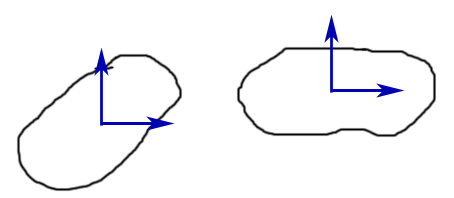
\includegraphics[width=0.30\textwidth]{softArt_G1.png}
	\caption{two bones}
	\label{2 Bones}
\end{figure}


Each of these bones contains several articulations points, also defined by rigids to have orientation information. \textsl{cf fig. 2}
\begin{figure}[htpb]
	\centering
		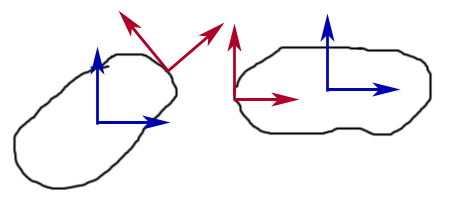
\includegraphics[width=0.30\textwidth]{softArt_G2.png}
	\caption{two bones (blue) with their articulation frames (red)}
\end{figure}

As seen previously, a joint between 2 bones is modeled by a 6-DOF spring. These springs are attached on the articulations points.    \textsl{cf fig. 3}
\begin{figure}[htpb]
	\centering
		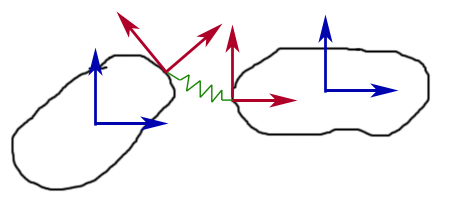
\includegraphics[width=0.30\textwidth]{softArt_G3.png}
	\caption{two bones linked by a joint-spring}
\end{figure}



\subsection{Sofa implementation}

To simulate these components in Sofa, we first need 2 mechanical objects : one for the bones (independent DOFs), and an other for the articulation points (mapped DOFs).
Each of them contains a list of rigid DOFs (respectively all the bones and all the articulations of the articulated body).
A mapping performs the link between the two lists, to know which articulations belong to which bones.


\subsubsection{Corresponding scene graph}
\begin{figure}[htpb]
	\centering
		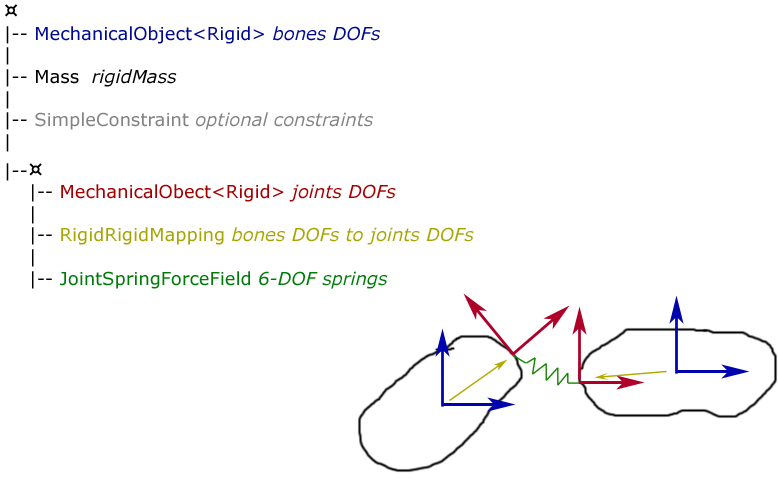
\includegraphics[width=0.90\textwidth]{scene_graph.png}
	\caption{a simple articulated body scene}
\end{figure}

\subsubsection {Example}

The example softArticulations.scn shows a basic pendulum :

\begin{verbatim}
<Node>
  <Object type="BruteForceDetection"/>
  <Object type="DefaultContactManager"/>
  <Object type="DefaultPipeline"/>
  <Object type="ProximityIntersection"/>

  <Node>
    <Object type="CGImplicitSolver"	/>
    <Object type="MechanicalObject" template="Rigid" name="bones DOFs"
            position="0 0 0  0 0 0 1 
                      1 0 0  0 0 0 1 
                      3 0 0  0 0 0 1 
                      5 0 0  0 0 0 1 
                      7 0 0  0 0 0 1" />
    <Object type="UniformMass" template="Rigid" name="bones mass"
            mass="1 1 [1 0 0,0 1 0,0 0 1]" />
    <Object type="FixedConstraint" template="Rigid" name="fixOrigin"
            indices="0" />
		
    <Node>
      <Object type="MechanicalObject" template="Rigid" name="articulation points"
              position="0 0 0  0.707914 0 0 0.707914 
                       -1 0 0  0.707914 0 0 0.707914 
                        1 0 0  0.707914 0 0 0.707914 
                       -1 0 0  0.707914 0 0 0.707914 
                        1 0 0  0.707914 0 0 0.707914 
                       -1 0 0  0.707914 0 0 0.707914 
                        1 0 0  0.707914 0 0 0.707914 
                       -1 0 0  0.707914 0 0 0.707914 
                        1 0 0  0.707914 0 0 0.707914" />
      <Object type="RigidRigidMapping"
              repartition="1 2 2 2 2" />
      <Object type="JointSpringForceField" template="Rigid" name="joint springs"
              spring="0 1   0 0 0 0 1 0   0 30000  0 200000   0  0 0 0  0 0 0 1 
                      2 3   0 0 0 0 1 0   0 30000  0 200000   0  0 0 0  0 0 0 1
                      4 5   0 0 0 0 1 0   0 30000  0 200000   0  0 0 0  0 0 0 1
                      6 7   0 0 0 0 1 0   0 30000  0 200000   0  0 0 0  0 0 0 1" />
    </Node>
    <Node>
      <Object type="MechanicalObject" template="Vec3d"
              position="-1 -0.5 -0.5  -1 0.5 -0.5 ..." />
      <Object type="MeshTopology"
              lines="0 1  1 2  ..."
              triangles="3 1 0  3 2 1  ..." />
      <Object type="TriangleModel"/>
      <Object type="LineModel"/>
      <Object type="RigidMapping"
              repartition="0 8 8 8 8" />
    </Node>
  </Node>
</Node>

\end{verbatim}

\begin{figure}[htpb]
	\centering
		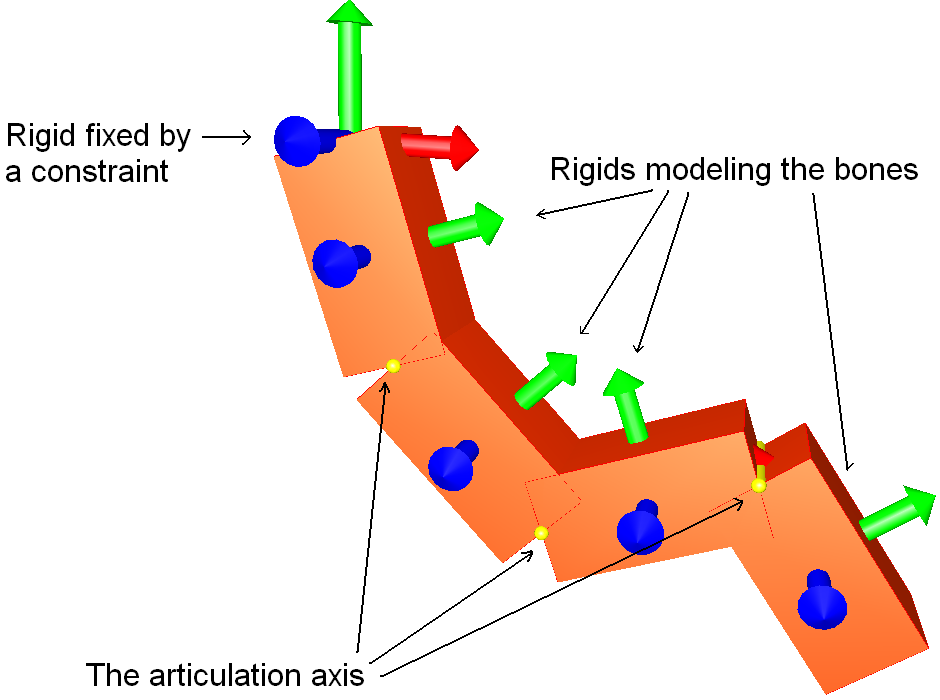
\includegraphics[width=0.70\textwidth]{softArt_snapshot.png}
	\caption{The pendulum is composed by 4 rigids linked one by one by articulations}
\end{figure}

In this example, we have under the first node the components to manage collisions, as usual.
Under the second node, we have :
\begin{itemize}
	\item the solver,
	\item the mechanical object modeling the independent rigid DOFs (5 rigids here),
	\item the rigid mass,
	\item a constraint, to fix the first rigid.
\end{itemize}

The third node (a child of the previous one) contains the components relative to the articulations :
\begin{itemize}
	\item the mechanical object modeling articulation points. Positions and orientations are relative to their parents.
	\item the mapping to link the two mechanical objects, as explained before. To know which articulations belong to which bones, a repartition vector is used. Several cases for this vector are possible :
		\begin{itemize}
			\item no value specified : every articulations belong to the first bone (classic rigid mapping).
			\item one value specified (ex: repartition="2") : each bone has the same number of articulations.
			\item number of bones values (like here, repartition="1 2 2 2 2") : the number of articulations is specified for each bone. For instance, here the first bone has 1 articulation, the next has 2 articulations, the next 2, Etc.
		\end{itemize}
	\item the JointSpringForceField containing the springs (4 springs here). Each spring is defined by a list of parameters. For instance for the first spring we have "0 1   0 0 0 0 1 0   0 30000  0 200000   0  0 0 0  0 0 0 1".
		\begin{itemize}
			\item "0 1" are the indices of the two articulations the spring is attached to
			\item "0 0 0 0 1 0" design the free axis for the movements. "0 0 0" mean that the 3 translation axis are constrained, and "0 1 0" mean that only the Y rotation axis is free.
			\item "0 30000 0 2000000" are the stiffnesses for each kind of movement: "0 30000" are respectively for free translation and for constrained translation", and "0 2000000" are respectively for free rotation and for constrained rotation.
			\item "0" is the damping factor
			\item "0 0 0" is to specify the initial translation
			\item "0 0 0 1" is to specify the initial rotation (quaternion)
		\end{itemize}
\end{itemize}

The last node contains the collision model. Nothing special here.


\subsection{Skinning}

The articulated body described previously models the skeleton of an object.
To have the external model (for the visual model or the collision model), which follows correctly the skeleton movements, it has to be mapped with the skeleton. 
\ 
A skinning mapping allows us to do this link. The external model is from this moment to deform itself smoothly, i.e. without breaking points around the articulations.

The influence of the bones on each point of the external model is given by skinning weights.
2 ways are possible to set the skinning weights to the mapping :
\begin{itemize}
	\item Either the user gives directly the weights list to the mapping. It is useful if good weights have been pre computed previsouly, like in Maya for instance.
	\item Else, the user defines a number of references \textsl{n} that will be used for mapped points. Then, each external model point will search its \textsl{n} nearest bones (mechanical DOFs), and then compute the skinning weights from the relation :
\[ W = \frac{1}{d^{2}}  \]
\small{ with \textsl{d} : the distance between the external point and the rigid DOF.}
\end{itemize}

\begin{figure*}[htpb]
		\centering
		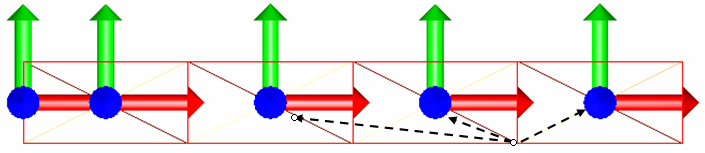
\includegraphics[width=0.50\textwidth]{skinning}
		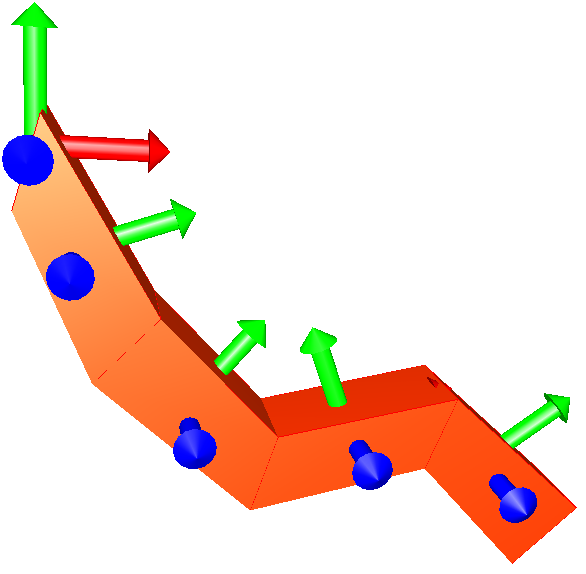
\includegraphics[width=0.30\textwidth]{skinnedPendulum}	
	\caption{In the example "softArticulationsSkinned.scn" the external points compute their skinning weights from the 3 nearest DOFs}
\end{figure*}

\newpage
\section{How to use mesh topologies in SOFA}

H. Delingette, B. Andr�

\subsection{Introduction}

\subsubsection{BTW, What is a mesh topology ?}

A mesh is usually described as a set of points that are connected by
edges, triangles or any other type of mesh element. Thus it is
useful to make a clear a distinction between two different aspects
of a mesh :

\begin{itemize}

 \item \textbf{Mesh Geometry} : the mesh geometry consists in the position of the mesh vertices.
This information depends on the space where the mesh in embedded.
For instance in a 2D triangulation, each vertex position is a 2D
vector while in a 3D triangulation, each vertex position is a 3D
vector. Therefore the mesh geometry can be described as an array of
vector whose size is the number of mesh vertices. In SOFA, we use
the word Degree Of Freedom (DOF) to describe such an array because
it can be used to store other geometric information (rigid
transformation, first or second derivatives, etc.).

 \item \textbf{Mesh Topology} : the mesh topology describes how the vertices are
connected with each other. For instance, it describes the set of
triangles by specifying the 3 vertex indices that make each
triangle. A mesh topology manipulates vertex indices (as unsigned
int) and therefore is independent of the embedding space. For
instance, a 2D and a 3D triangulation may have the same mesh
topology but with different mesh geometry.

\end{itemize}


\subsubsection{Why do I need to bother with mesh topologies ?}

As discuss above, mesh topology is an essential part of a mesh and
therefore any computation task that requires a mesh needs to know
how to use a mesh topology.\\ This includes:

\begin{itemize}

 \item \textbf{Mesh Visualization},

 \item \textbf{Collision detection} : some collision detection are mesh based (e.g.
triangles or edges),

 \item \textbf{Mechanical Modeling} : deforming a mesh also requires to the
knowledge of a mesh topology. For instance a spring mass model
requires knowing about the edges that connects pair of vertices,

 \item \textbf{Haptic rendering},

 \item \textbf{Description of scalar} (temperature, electric potential, etc.) or
vectorial fields (speed, fiber orientation, etc.)

\end{itemize}

Using a mesh topology is relatively simple since it consists in
having access to arrays of indices corresponding to vertex indices
or edge indices or other topological items.
\\

A more tricky part consists a) in changing locally or globally this
topology (adding a triangle, removing an edge) and b) in propagating
those changes to all objects using the mesh topology to perform a
task (visualization, deformation, etc.)

\subsubsection{How are Mesh Topologies designed in SOFA ?}

The mesh geometry in SOFA is stored in a MechanicalObject which is a
template class because it depends on the embedding space (2D or 3D
Euclidian space), the vector class and the required floating point
accuracy (float vs double).
\\

A mesh topology is stored in a different object than the mesh
geometry.
\\

One important aspect of the design of mesh topologies in SOFA is the
fact that they are organized in a class hierarchy. For instance, a
triangulation object derives from an edge set object since a
triangulation can be also viewed as a set of edges, each triangle
having 3 edges. This is very important to design generic software
components. Indeed, following the same example, with this design, a
spring mass mechanical model that only requires the knowledge of
edges (pairs of vertices) can also be used on a triangulation or any
other mesh (quad, hexahedral, tetrahedral mesh)  that derives from
an edge set object.
\\

Another interesting feature in SOFA is the ability to provide
multiple topology descriptions for the same mesh. For instance a
quad element (see figure below) has four DOFs which can be connected
with 2 triangles or 6 edges. Thus, the same mesh geometry can be
described by 3 different mesh topologies. SOFA uses the mechanism of
topological mapping to provide multiple topologies associated with
the same mesh geometry. Those mappings also apply to map a subset of
the mesh topology into a new mesh topology.  For instance the border
of a tetrahedral mesh can be mapped into triangulation mesh or edges
of a triangulated mesh can be mapped into a polygonal mesh.\\


\begin{figure*}
 \centering
 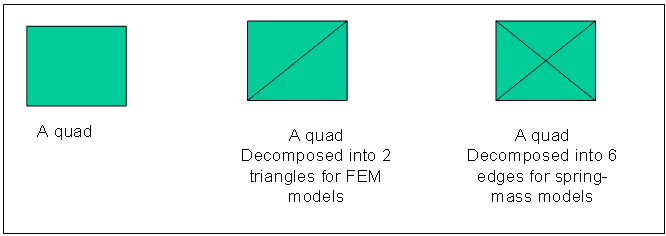
\includegraphics[width=0.95\linewidth]{Quad_Multiple_Topologies}
  \caption{Multiple topology descriptions of the Quad.}
 \label{fig:Quad_Multiple_Topologies}
\end{figure*}

Another important aspect of the design is the fact that topological
changes (mesh cutting or refinement) are handled in SOFA.  For the
programmer, it implies that specific containers must be used to
store data for each software component. For instance, a spring mass
model must store the spring stiffness of each edge. Therefore the
container of spring stiffness must have the same size than the
number of edges in the mesh. In SOFA, to cope with topological
changes that can add or remove the number of edges, it is mandatory
to use a specific container (in such case EdgeData container) that
will automatically resize itself when topological changes occur.

\subsubsection{What are the different mesh topologies supported in SOFA ?}


\subsection{Using Mesh Topologies}

\subsubsection{What is a mesh topology object ?}
\subsubsection{What is the difference with the old MeshTopology object ?}
\subsubsection{What are the different mesh topology objects in SOFA ?}


\begin{figure*}
 \centering
 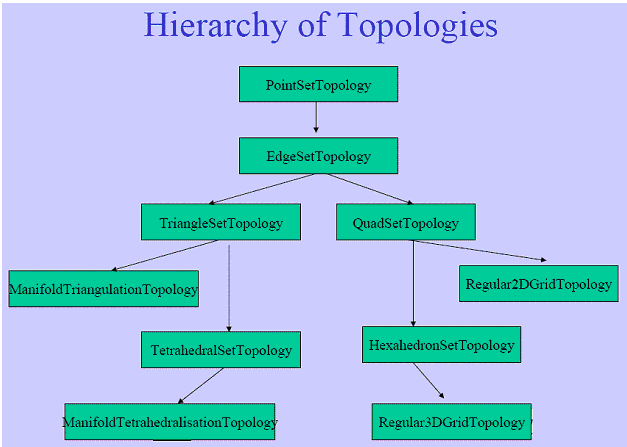
\includegraphics[width=0.95\linewidth]{Hierarchy_Topologies}
  \caption{A generic and hierarchical topology is described from a class called BaseTopology.}
 \label{fig:Hierarchy_Topologies}
\end{figure*}

BaseTopology class provides an implementation which handles
topological changes, full topological relationships and geometric
computation.

\subsubsection{How do I have access to the adjacency information between items ?}
\subsubsection{What to do if I need to know only basic topology information ?}
\subsubsection{What are the geometry algorithms stored in each topology classes ?}

\subsection{Handling Topological Changes}

\subsubsection{How does it work ?}
\subsubsection{What container should I use to handle the topology changes ?}
\subsubsection{How to write the different callback functions associated with the containers ?}

Topological changes are handled in a way which is as much
transparent for the user as possible.


\subsubsection{The 4 components of a BaseTopology object}

\begin{verbatim}

Class BaseTopology<DataTypes> {

// A container for info to be stored and methods to access adjacency :
//   - Adjacency Information is only computed when needed
//   - Non template class
//   - Store TopologicalChange list

TopologyContainer *container ;

// A modifier for low-level methods to change topology :
//   - Cannot be accessed from user
//   - Modifier also changes the DOFs in the Mechanical Object
//   - Low level methods to add or to remove an item
TopologyModifiers<DataTypes> *modifier ;

// TopologyAlgorithms for high-level methods to change topology (user access) :
//   - Accessed from the user
//   - High level algorithms to refine, cut mesh
TopologyAlgorithms<DataTypes> *topologyAlgorithms ;

// Geometry Algorithms methods to get geometry information :
//   - Compute geometric information (normal, curvature, area, length)
GeometryAlgorithms<DataTypes> *geometryAlgorithms ;

};

\end{verbatim}


\subsubsection{Implementation for objects inherited from each other (Point,
Edge, Triangle, Tetrahedron}


\begin{itemize}

 \item PointSetTopology (inherited from BaseTopology) :

    \begin{itemize}

    \item Container : For each point gives its global index. This is useful for subset topologies (subset triangulation, ...) where the number of vertices involved in the topology may not be the same as the total number of vertices.

    \item Modifier : addPointsProcess, removePointsProcess, renumberPointsProcess, addPointsWarning, removePointsWarning, propagateTopologicalChanges

    \item Geometry : computeCenter, computeRadius,
    getAABB()

    \end{itemize}


\item EdgeSetTopology (inherited from PointSetTopology)

    \begin{itemize}

    \item Container : array of edges, array of vertex-edge shell

    \item Modifier : addEdgesProcess, removeEdgesProcess, fuseEdgesProcess, splitEdgesProcess,
   addEdgesWarning, removeEdgesWarning

    \item Geometry : getEdgeLength, getRestEdgeLength

    \end{itemize}


\item TriangleSetTopology (inherited from EdgeSetTopology)

    \begin{itemize}

    \item Container : array of triangles, of vertex- and edge-triangle shell

    \item Modifier : addTrianglesProcess, removeTrianglesProcess, addTrianglesWarning, removeTrianglesWarning

    \item Topology Algorithms : InciseAlongPointsList, RemoveAlongTrianglesList

    \item Geometry : computeTriangleNormal

    \end{itemize}


\item TetrahedronSetTopology (inherited from TriangleSetTopology)

    \begin{itemize}

    \item Container : array of tetrahedra, array of vertex-, edge-, triangle-tetrahedra shell

    \item Modifier : addTetrahedraProcess, removeTetrahedraProcess, addTetrahedraWarning, removeTetrahedraWarning

    \item Geometry : computeTetrahedronVolume

    \end{itemize}

\end{itemize}

\begin{figure*}
 \centering
 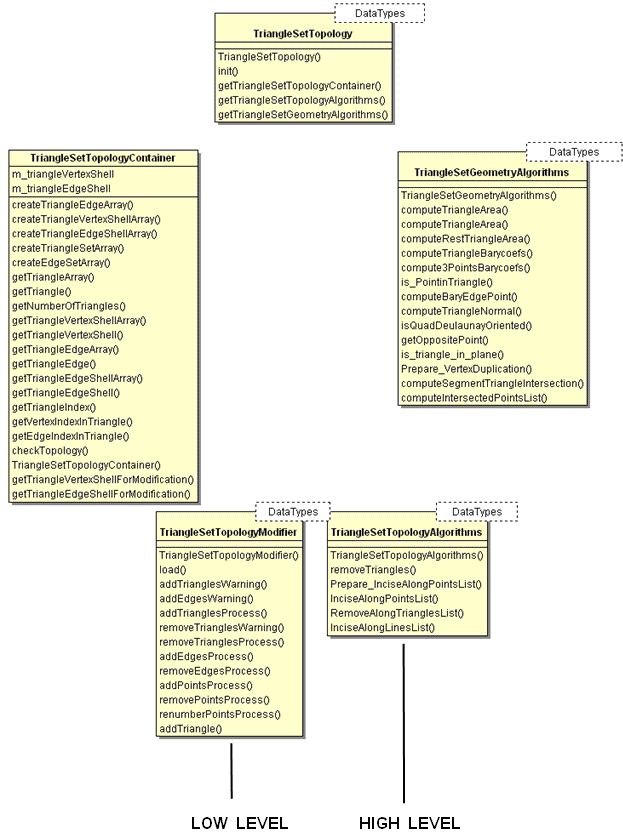
\includegraphics[width=0.95\linewidth]{UML_TriangleSetTopology}
  \caption{UML diagram describing the 4 components of TriangleSetTopology class.}
 \label{fig:UML_TriangleSetTopology}
\end{figure*}

\newpage

\begin{figure*}
 \centering
 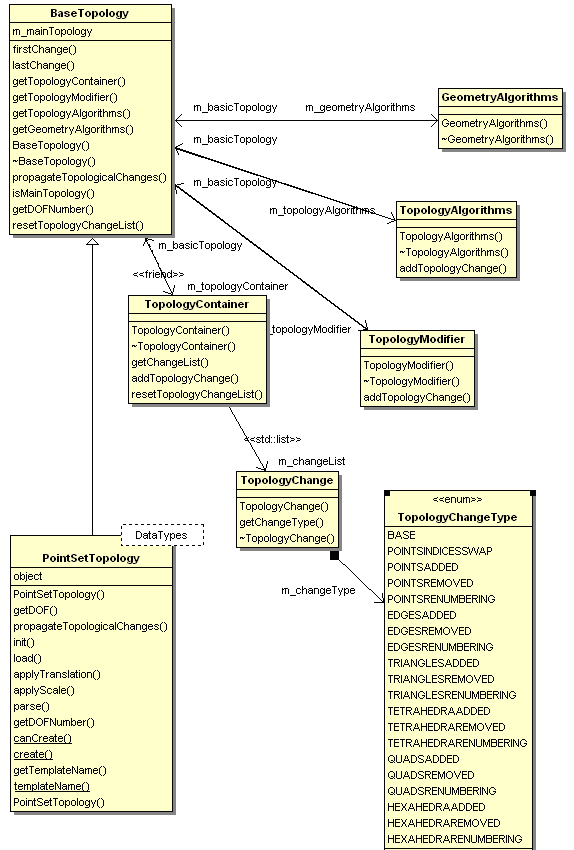
\includegraphics[width=0.95\linewidth]{UML_BaseTopology}
  \caption{UML diagram showing the use of a TopologyChanges List from BaseTopology class.}
 \label{fig:UML_BaseTopology}
\end{figure*}

\newpage

\subsubsection{Definition of data structures to be "aware" of topological
changes}

Force Fields, Constraints, Mapping and other modules may require to
store information for each topological item (point, edge, triangle,
etc.).
\\

Two container data structures are defined to handle topological
changes by matching the types of TopologyChanges :

\begin{itemize}

    \item PointData$<$MyType$>$, EdgeData$<$MyType$>$ are arrays (same as std::vector) of item of type MyType

    \item PointSubset, EdgeSubset are arrays of points or edges

\end{itemize}

Used-defined functions are called when an item is created or
destroyed.
\\

In higher level classes (for example
TriangularQuadraticSpringForceField, DiagonalMass or FixedConstraint
classes), the user only provides callback functions to handle :

\begin{itemize}

    \item the creation of a topological item
    \item the destruction of a topological item

\end{itemize}

\begin{figure*}
 \centering
 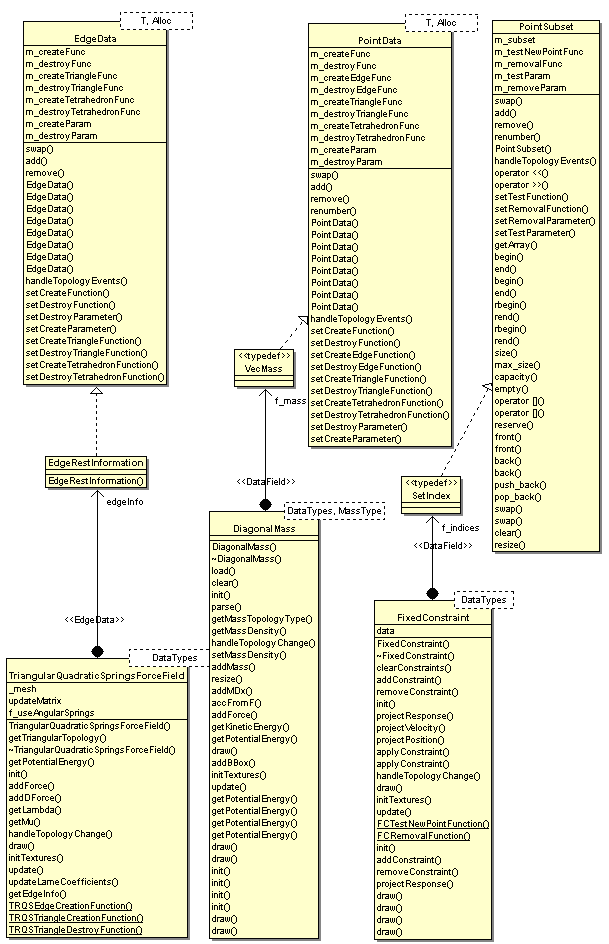
\includegraphics[width=0.95\linewidth, height=0.95\textheight]{UML_Topological_Changes}
  \caption{These UML diagrams show the use of EdgeData, PointData and
PointSubset to handle topological changes implying modifications
respectively in ForceField, Mass and Constraint modules.}
 \label{fig:UML_Topological_Changes}
\end{figure*}

\newpage

\begin{figure*}
 \centering
 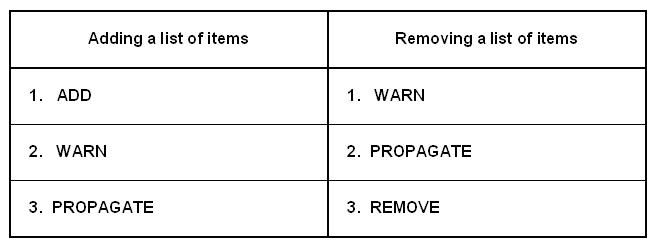
\includegraphics[width=0.95\linewidth]{Order_Notifications}
  \caption{Order to respect when adding or removing an item (see the
explanations in the following example).}
 \label{fig:Order_Notifications}
\end{figure*}

\begin{itemize}

    \item "WARN" means : add the current topological change (add or delete a list of items) in the list of TopologyChanges

    \item "PROPAGATE" means :  traverse the simulation tree with a TopologyChangeVistor to send
    the current topological change event to all force fields, constraints,
    mappings, etc.

\end{itemize}

\subsubsection{Example : What happens when I split an Edge ?}

\begin{figure*}
 \centering
 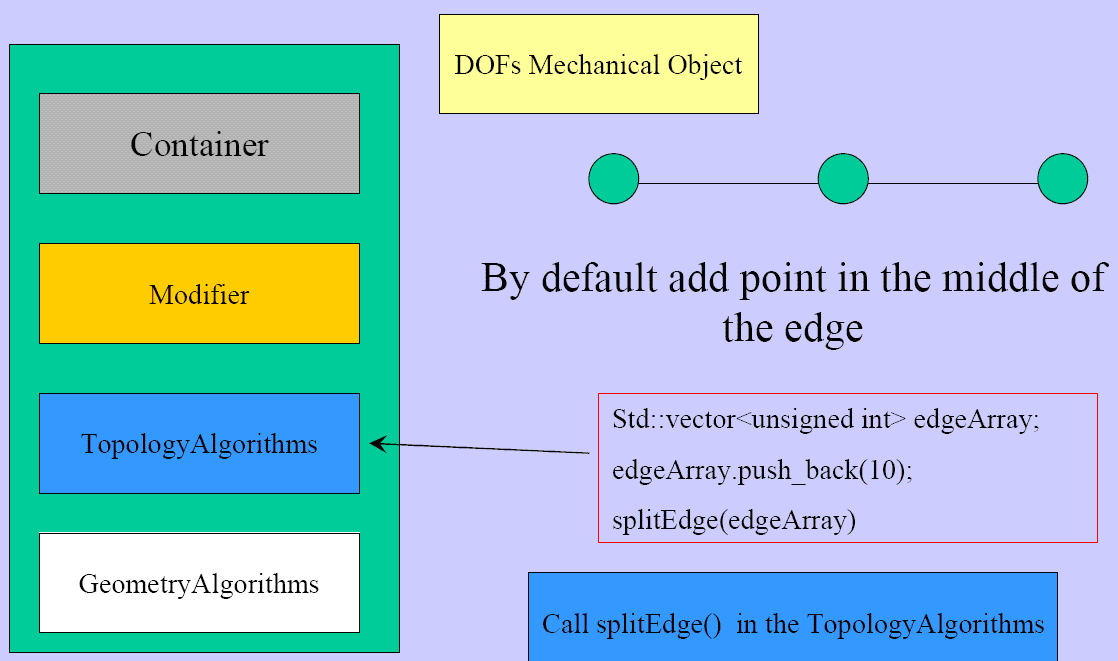
\includegraphics[width=0.95\linewidth]{Topology_Example_1}
 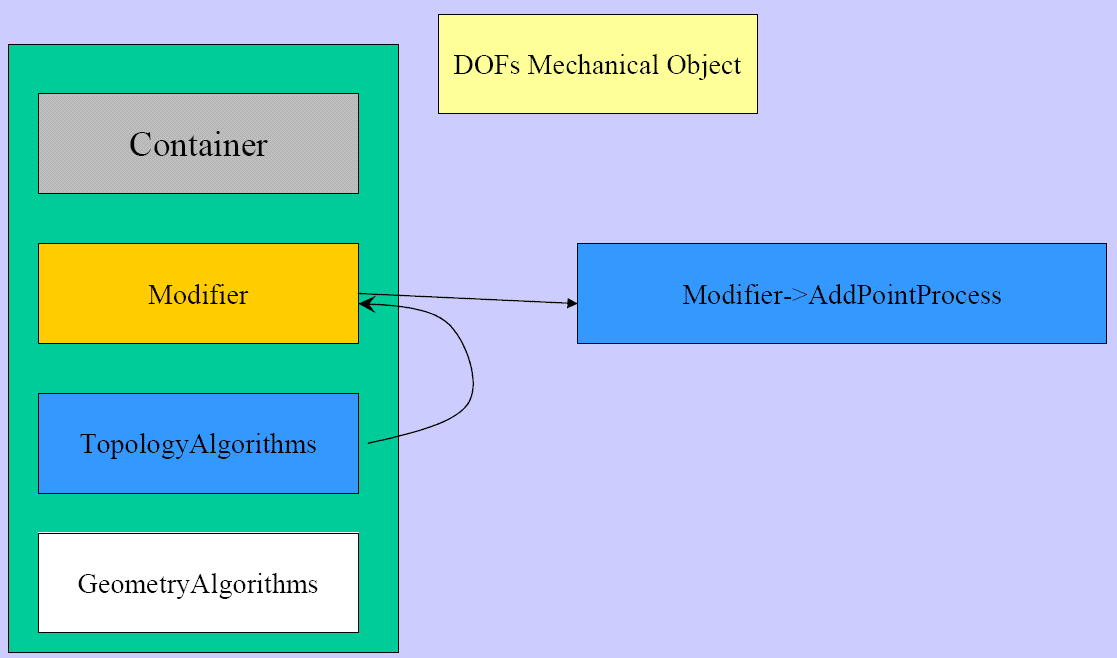
\includegraphics[width=0.95\linewidth]{Topology_Example_2}
  \caption{What happens when I split an Edge ? - Step 1. 2.}
 \label{fig:Topology_Example_12}
\end{figure*}

\newpage

\begin{figure*}
 \centering
 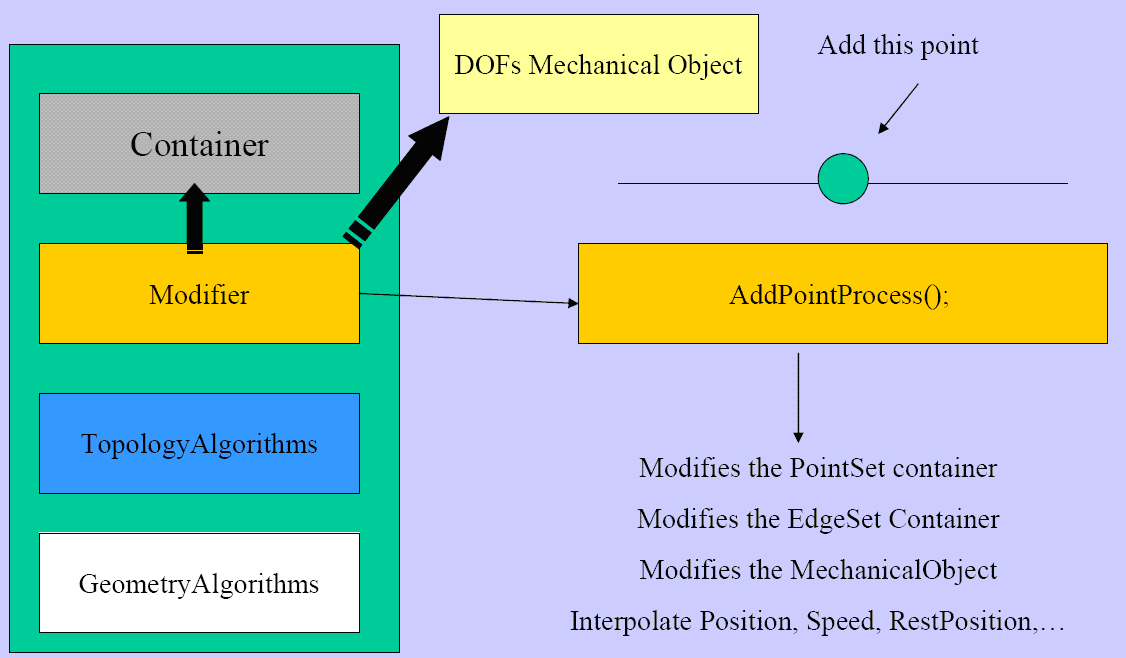
\includegraphics[width=0.95\linewidth]{Topology_Example_3}
 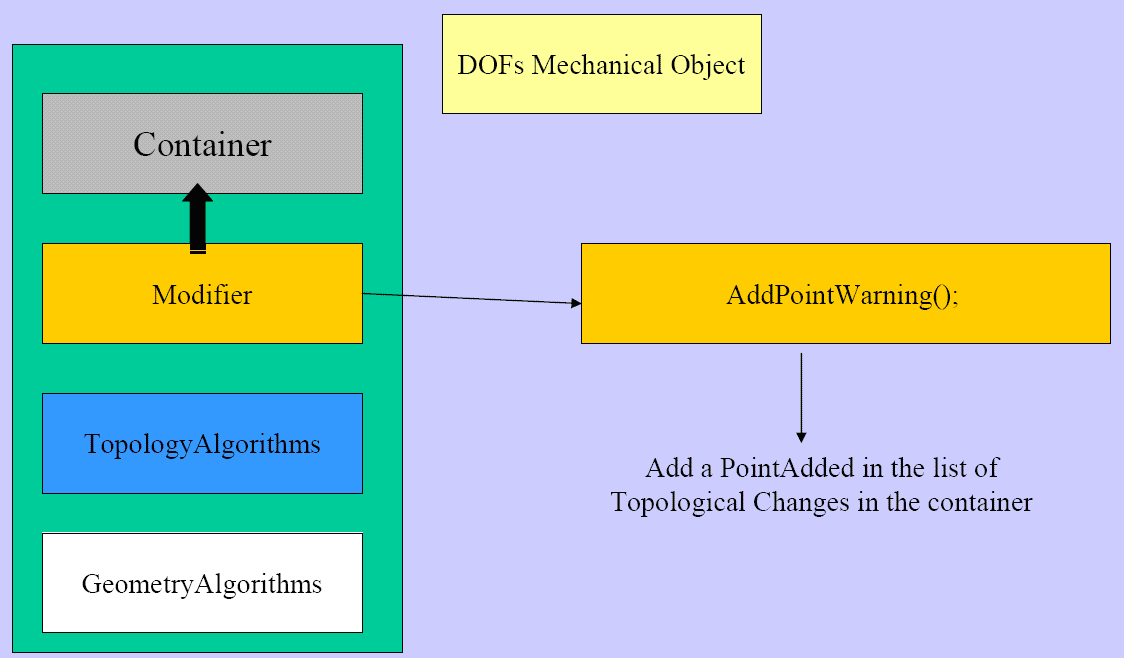
\includegraphics[width=0.95\linewidth]{Topology_Example_4}
  \caption{What happens when I split an Edge ? - Step 3. 4.}
 \label{fig:Topology_Example_34}
\end{figure*}

\newpage

\begin{figure*}
 \centering
 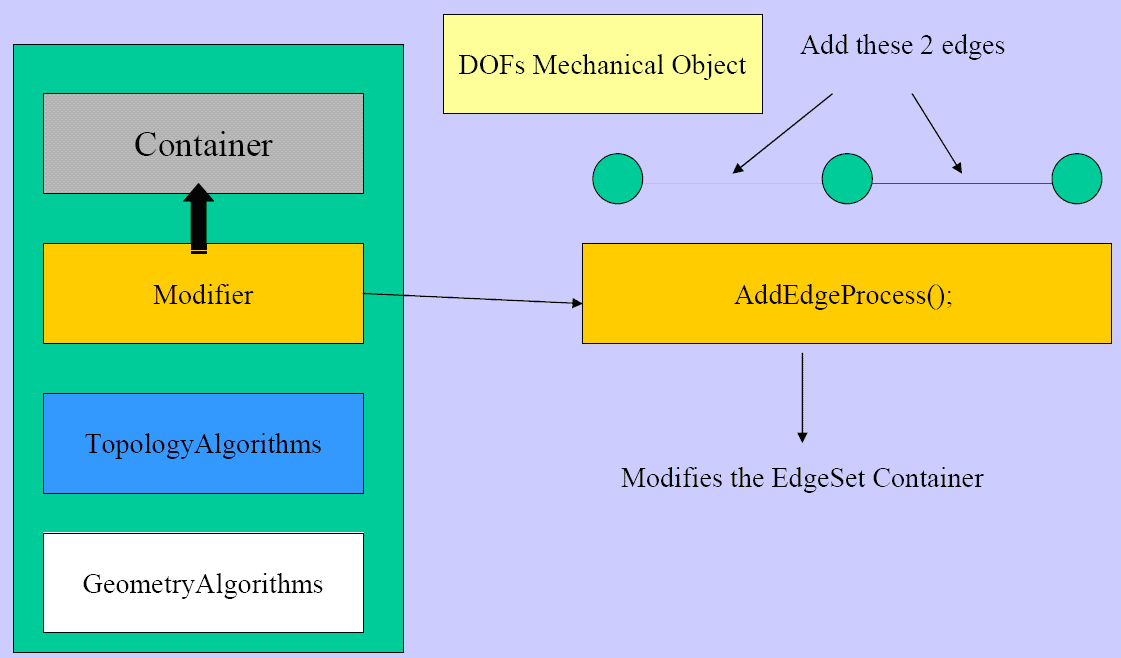
\includegraphics[width=0.95\linewidth]{Topology_Example_5}
 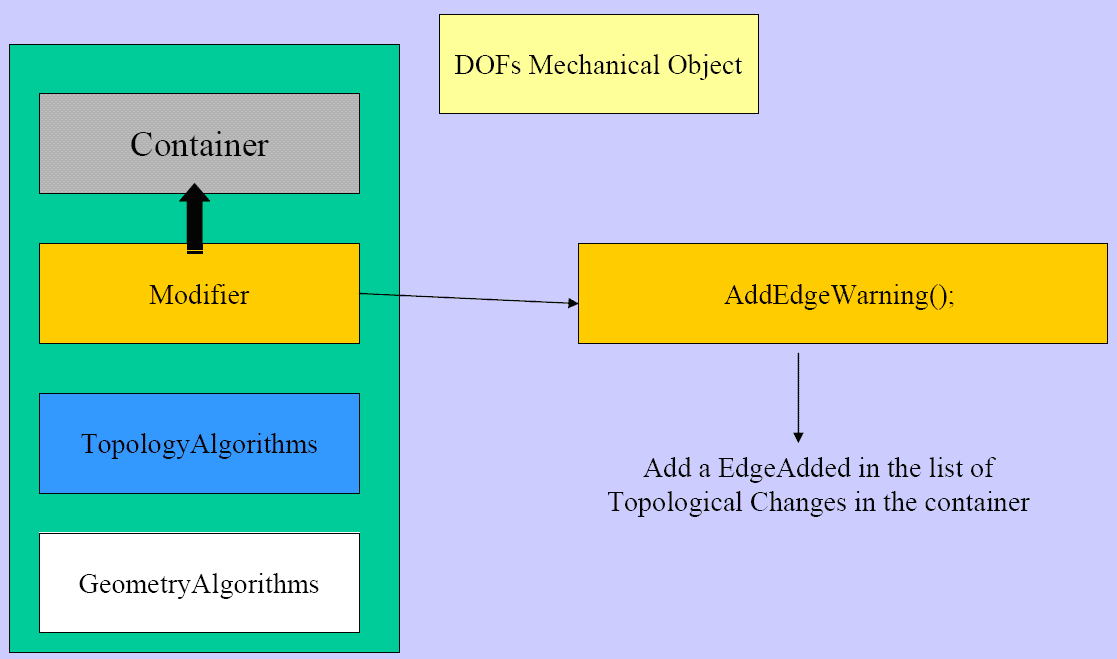
\includegraphics[width=0.95\linewidth]{Topology_Example_6}
  \caption{What happens when I split an Edge ? - Step 5. 6.}
 \label{fig:Topology_Example_56}
\end{figure*}

\newpage

\begin{figure*}
 \centering
 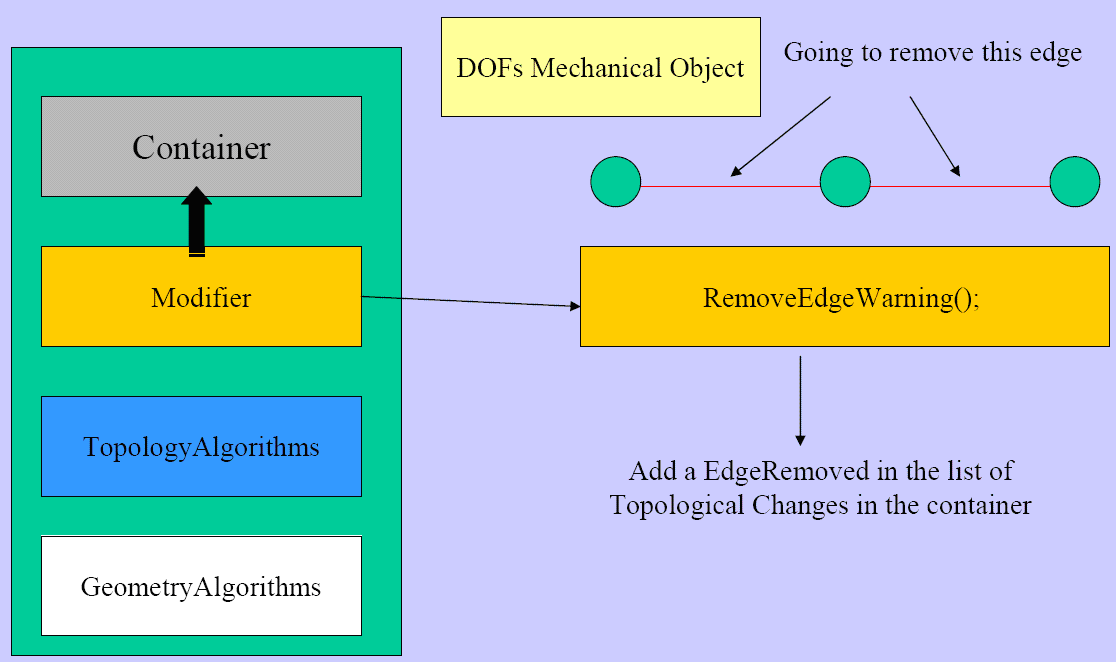
\includegraphics[width=0.95\linewidth]{Topology_Example_7}
 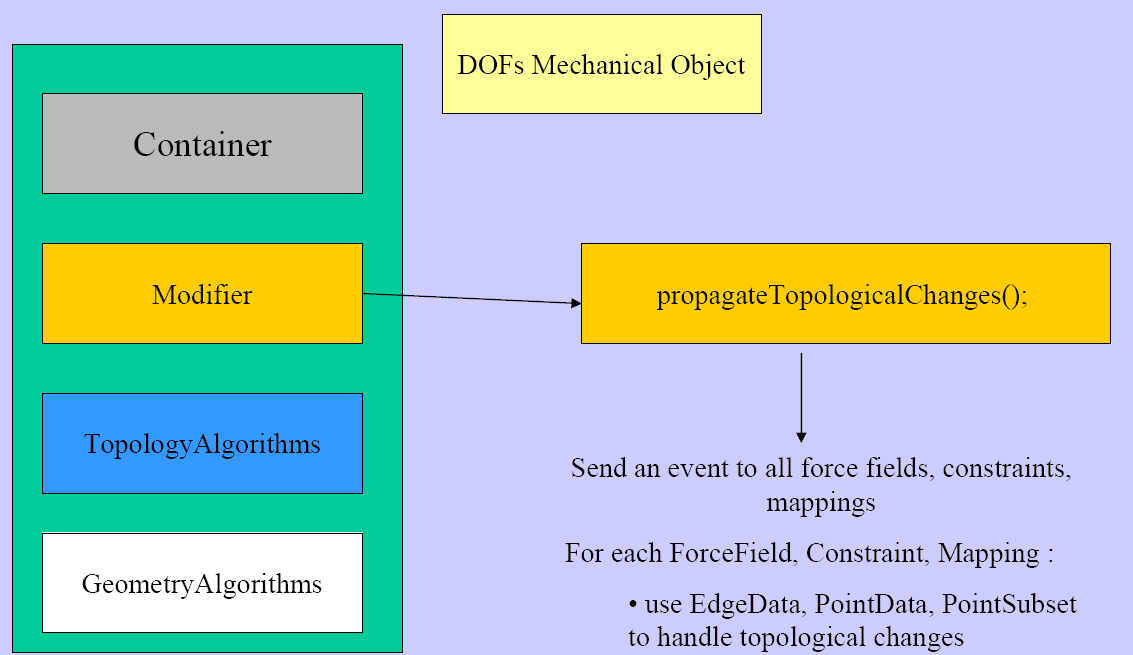
\includegraphics[width=0.95\linewidth]{Topology_Example_8}
  \caption{What happens when I split an Edge ? - Step 7. 8.}
 \label{fig:Topology_Example_78}
\end{figure*}

\newpage

\begin{figure*}
 \centering
 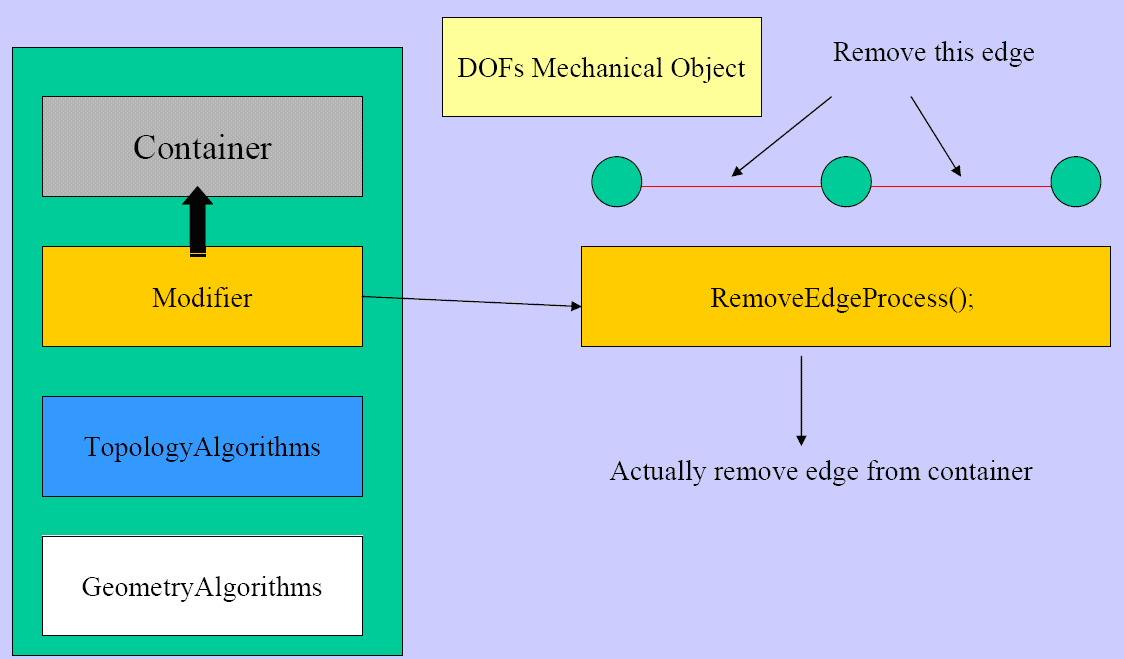
\includegraphics[width=0.95\linewidth]{Topology_Example_9}
  \caption{What happens when I split an Edge ? - Step 9.}
 \label{fig:Topology_Example_9}
\end{figure*}



\end{document}          

